% 20190826
% It will be increased by 1 after \chapter
\setcounter{chapter}{0}
% Set this page number
\setcounter{page}{1}


\chapter{Pendahuluan}
Secara umum banyak sistem fisis yang dapat dimodelkan dengan menggunakan butiran-butiran yang saling berinteraksi baik secara permanen (rentang jauh) ataupun hanya sesekali (rentang dekat). Tulisan ini akan membahas hal tersebut yang dilengkapi dengan contoh implementasinya menggunakan pustaka \verb|butiran.js|\footnote{url \url{https://github.com/dudung/butiran.js} [20191017]} yang ditulis dalam bahasa pemrograman JavaScript (JS).


%
\section{Berkas-berkas utama}
Terdapat beberapa berkas yang diperlukan untuk menjalankan pustaka \verb|butiran.js|, yaitu berkas HTML dan JS yang dalam contoh ini bernama \verb|hello.html| dan \verb|hello.js|, serta versi terkompresi dari pustaka tersebut dengan nama berkas \verb|butiran.min.js| yang dapat diperoleh dari folder \verb|dist|.

\lstinputlisting[label={lst:hello.html}, caption={Berkas {\tt hello.html}.}, linerange={1}, firstnumber=1]{01/hello.html}

Kode \ref{lst:hello.html} memerlukan dua berkas yaitu versi terkompresi dari pustaka \verb|butiran.js| dan berkas \verb|hello.js|.

\lstinputlisting[label={lst:hello.js}, caption={Berkas {\tt hello.js}.}, linerange={1}, firstnumber=1]{01/hello.js}

Isi dari berkas \verb|hello.js| diberikan dalam Kode \ref{lst:hello.js}. Beris 18 akan menuliskan frasa "Hello world!" pada konsol perambat internet, e.g. Google Chrome, baris 19 mendefinisikan suatu besaran berjenis \verb|Vect3| dan baris 20 menuliskan isinya. Kelas \verb|Vect3| merupakan bagian dari pustaka \verb|butiran.js| yang bila tidak ada pesan kesalahan menunjukkan bahwa pustaka ini telah sukses disertakan.

\begin{figure}[H]
\centering
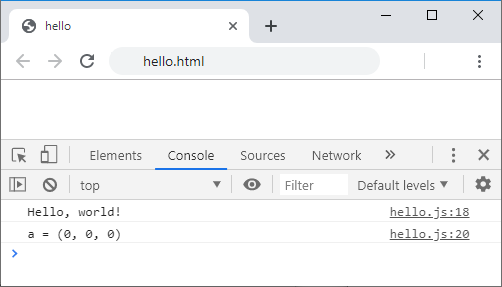
\includegraphics[width=10cm]{01/hello.png}
\caption{\label{fig:hello} Tampilan berkas {\tt hello.html} dalam peramban internet Google Chrome.}
\end{figure}

Untuk melihat konsol pada Google Chrome digunakan kombinasi tombol CTRL + SHIFT + J, yang berbeda-beda untuk setiap peramban internet.\footnote{"How to open the developer console", Airtable, url \url{https://support.airtable.com/hc/en-us/articles/232313848-How-to-open-the-developer-console} [20191017].} Dalam Gambar \ref{fig:hello} pada bagian kanan tercantum baris keberapa pada berkas \verb|hello.js| yang menghasilkan keluaran tersebut. Dengan menggunakan informasi ini pengguna dapat melacak hasil keluaran yang diperoleh.

Untuk berikutnya terkait dengan konsol bila tidak benar-benar diperlukan tampilan dalam peramban internet tidak akan ditayangkan, melainkan cukup hanya bagian teksnya tersebut

\begin{lstlisting}[numbers=none]
Hello, world!                                  hello.js:18
a = (0, 0, 0)                                  hello.js:20
\end{lstlisting}

yang ditampilkan.


%
\section{Catatan}
Rujukan, terutama yang yang bersumber dari internet, akan disertakan sebagai catatan kaki.